\documentclass[11pt]{article}

\usepackage[margin=1in]{geometry}
\usepackage[utf8]{inputenc}
\usepackage[T1]{fontenc}
\usepackage{graphicx}
\usepackage{booktabs}
\usepackage{array}
\usepackage{longtable}
\usepackage{float}
\usepackage{amsmath}
\usepackage[version=4]{mhchem}
\usepackage{siunitx}
\usepackage{url}
\usepackage{xspace}

\graphicspath{{../figures/}{../si_figures/}{figures/}{si_figures/}}
\renewcommand{\thefigure}{S\arabic{figure}}
\renewcommand{\thetable}{S\arabic{table}}
\newcommand{\waterair}{water--air\xspace}
\newcommand{\sfg}{SFG\xspace}
\newcommand{\imchi}{\ensuremath{\mathrm{Im}\,\chi^{(2)}}\xspace}

\title{\textbf{Supplementary Material}\\
The Silica/Water Interface Revisited: Elucidating Interfacial Water Structure with an SFG Rosetta Stone}
\author{Jen{\'e}e D. Cyran and Thomas D. K{\"u}hne}
\date{}

\begin{document}
\maketitle

\section*{Overview}

This Supporting Information documents the silica/water SFG analysis in the main text. The experimental data contain one response channel on the corresponding frequency axis. The structural fits are performed directly on the experimental trace after 17-point moving-average smoothing.

The central model in the main text is the three-motif I+VI+VIII fit in the \SIrange{3300}{3800}{cm^{-1}} window. This is treated as the primary physically interpretable OH-transfer window, not as the only valid spectral interval. The window choice is derived from the experimental trace and the model-selection diagnostics rather than from an external structural assignment. The broader \SIrange{3200}{3800}{cm^{-1}} interval is used diagnostically to expose low-edge sensitivity. The \SIrange{3400}{3800}{cm^{-1}} interval is used as a high-frequency control, where the trace is numerically clean but less discriminating because several related bridge-family models fit it almost equally well. The \SIrange{3300}{3800}{cm^{-1}} window is therefore the best balance between data quality and structural information.

All structural fits use nonnegative weights, a floating linear baseline, a global frequency shift, and a global sign convention. The sign parameter is bookkeeping for comparing digitized fingerprints. The structural interpretation follows the silica-side viewing convention used in the main text, where positive \imchi corresponds to OH/H orientation toward \ce{SiO2}. The reported weights are coherent RMS-normalized fingerprint contributions. They are not molecule counts. Direct L3-control fits compare VII- and VIII-containing models in order to test whether the deeper-layer response is best represented by motif VIII alone or by an VIII-dominated mixture with motif VII.

\section*{Experimental Trace}

\begin{figure}[H]
\centering
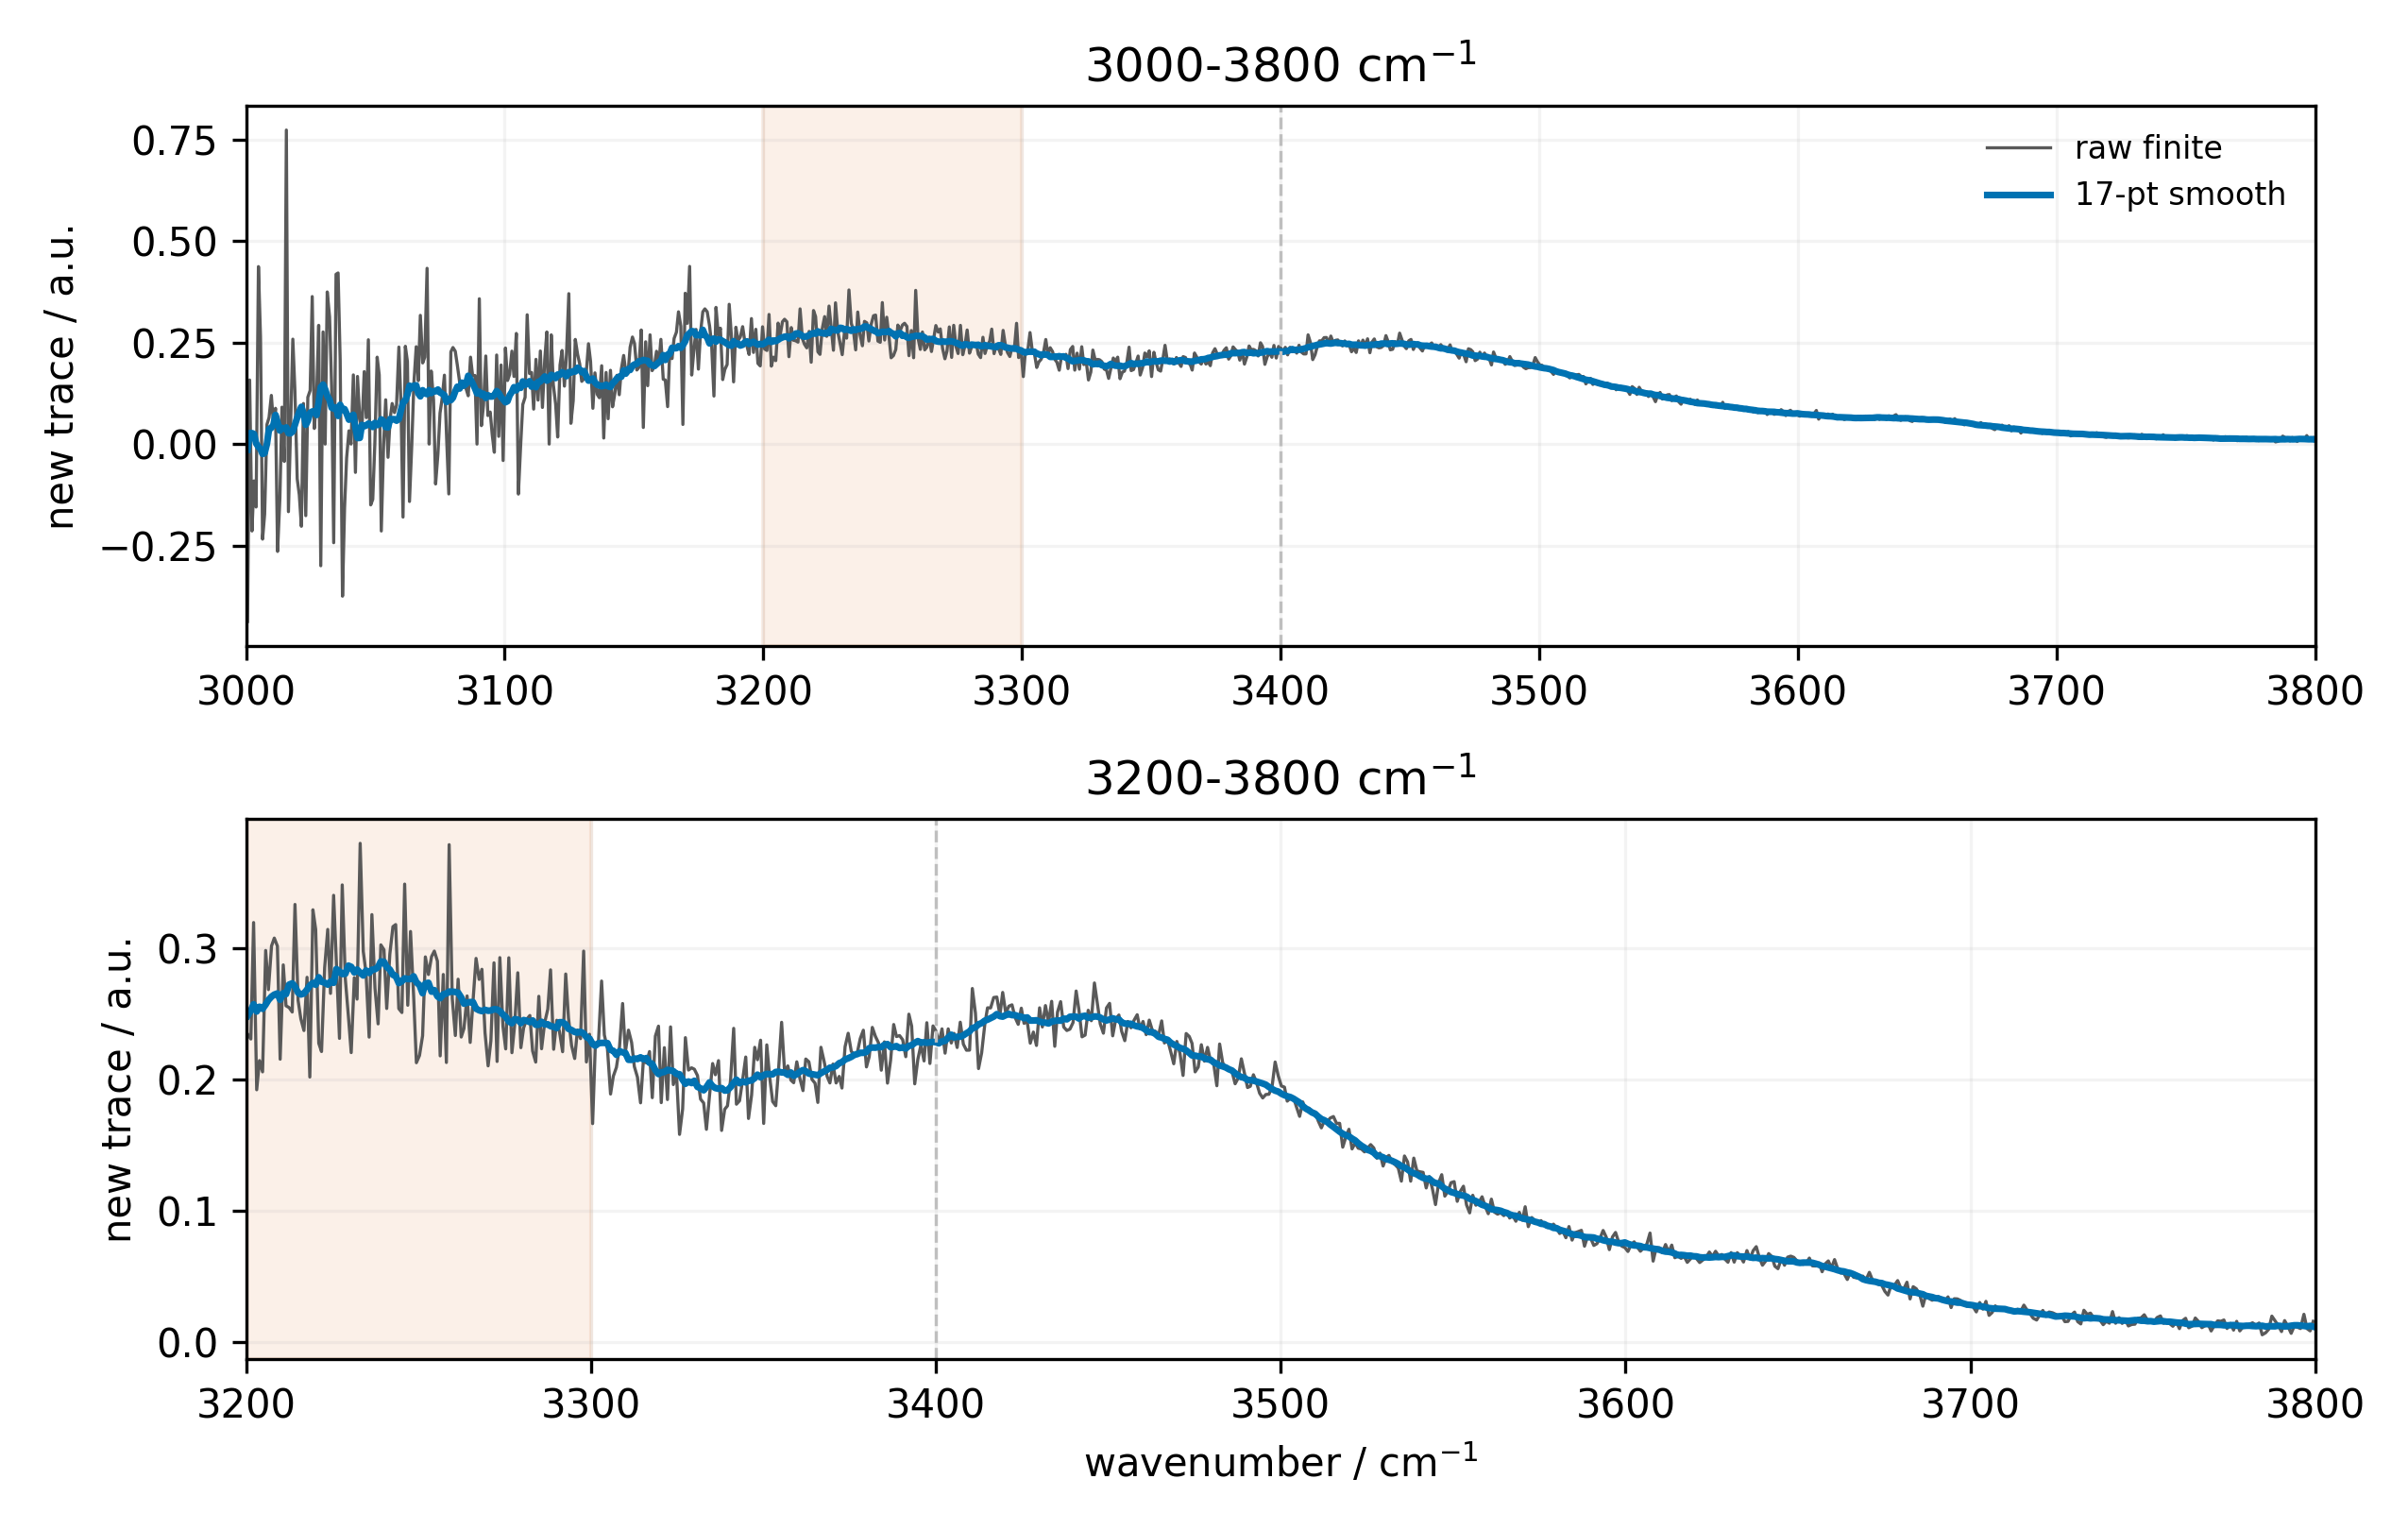
\includegraphics[width=0.92\textwidth]{figS_new_trace_usable_zoom}
\caption{Experimental trace and 17-point moving-average smoothing. The \SIrange{3200}{3300}{cm^{-1}} interval is shown as a low-edge noise caution region. The primary physically interpretable OH-transfer window used in the main text is \SIrange{3300}{3800}{cm^{-1}}.}
\end{figure}

The source file contains 1600 frequency points. Of these, 1578 are finite. The 22 nonfinite values occur between \SI{2674.4}{cm^{-1}} and \SI{2883.5}{cm^{-1}}, outside the structural OH-stretch window used for the Rosetta-stone fits. The trace is finite throughout all windows from \SI{3000}{cm^{-1}} upward.

\begin{table}[H]
\centering
\caption{Data-internal window-choice diagnostics for the experimental trace. The raw-minus-smoothed RMS is computed from the finite raw trace and the 17-point smoothed trace. The relative point-noise estimate is this RMS divided by the local peak-to-peak amplitude of the smoothed trace.}
\begin{tabular}{lcccc}
\toprule
window / \si{cm^{-1}} & role & points & RMS / a.u. & relative noise \\
\midrule
3000--3200 & low-frequency noisy region & 237 & 0.1380 & 0.451 \\
3200--3300 & low-edge noise caution & 116 & 0.0359 & 0.610 \\
3300--3800 & primary OH-transfer window & 557 & 0.0104 & 0.044 \\
3400--3800 & high-frequency control & 443 & 0.0064 & 0.027 \\
3350--3700 & narrow peak-shape control & 392 & 0.0088 & 0.040 \\
\bottomrule
\end{tabular}
\end{table}

The \SIrange{3300}{3800}{cm^{-1}} window is therefore a compromise rather than a fitted convenience. It avoids the high relative point noise at the low edge, while retaining more of the bonded-OH response than the \SIrange{3400}{3800}{cm^{-1}} high-frequency control. The \SIrange{3200}{3800}{cm^{-1}} window is retained as a diagnostic control because it tests how strongly the fit responds to the noisier lower edge. In this sense, the primary OH-transfer window is selected by the measured trace and by structural discriminability, not by imposing the silica/water interpretation of Cyran \textit{et al.}

\section*{Primary Model and Four-Motif Control}

\begin{table}[H]
\centering
\caption{Primary model selection in the \SIrange{3300}{3800}{cm^{-1}} window using 17-point smoothing and a conservative global shift range of \SI{\pm20}{cm^{-1}}.}
\begin{tabular}{lcccccc}
\toprule
model & active motifs & $R^2$ & SSE & shift / \si{cm^{-1}} & sign & BIC \\
\midrule
primary three-motif & I+VI+VIII & 0.995350 & 0.019173 & +4 & +1 & -5692.6 \\
four-motif control & I+VI+VII+VIII & 0.995433 & 0.018829 & +2 & +1 & -5696.3 \\
\bottomrule
\end{tabular}
\end{table}

The four-motif control gives a slightly smaller residual, but the numerical gain is small relative to the physical cost of adding another L3 motif. The main text therefore uses I+VI+VIII as the parsimonious three-motif structural model and discusses VII as a symmetry-related/near-degenerate admixture that cannot be uniquely excluded.

\begin{table}[H]
\centering
\caption{RMS-normalized fingerprint fractions for the primary I+VI+VIII fit. These values are spectral weights, not molecular populations.}
\begin{tabular}{llcc}
\toprule
motif & role & nonnegative weight & RMS fraction \\
\midrule
I & L1 weak/free-OH marker & 0.002610 & 0.0234 \\
VI & L2 bridge-family connector & 0.021721 & 0.1948 \\
VIII & L3 bonded-water response & 0.087150 & 0.7817 \\
\bottomrule
\end{tabular}
\end{table}

\section*{Direct L3 VII/VIII Control}

\begin{figure}[H]
\centering
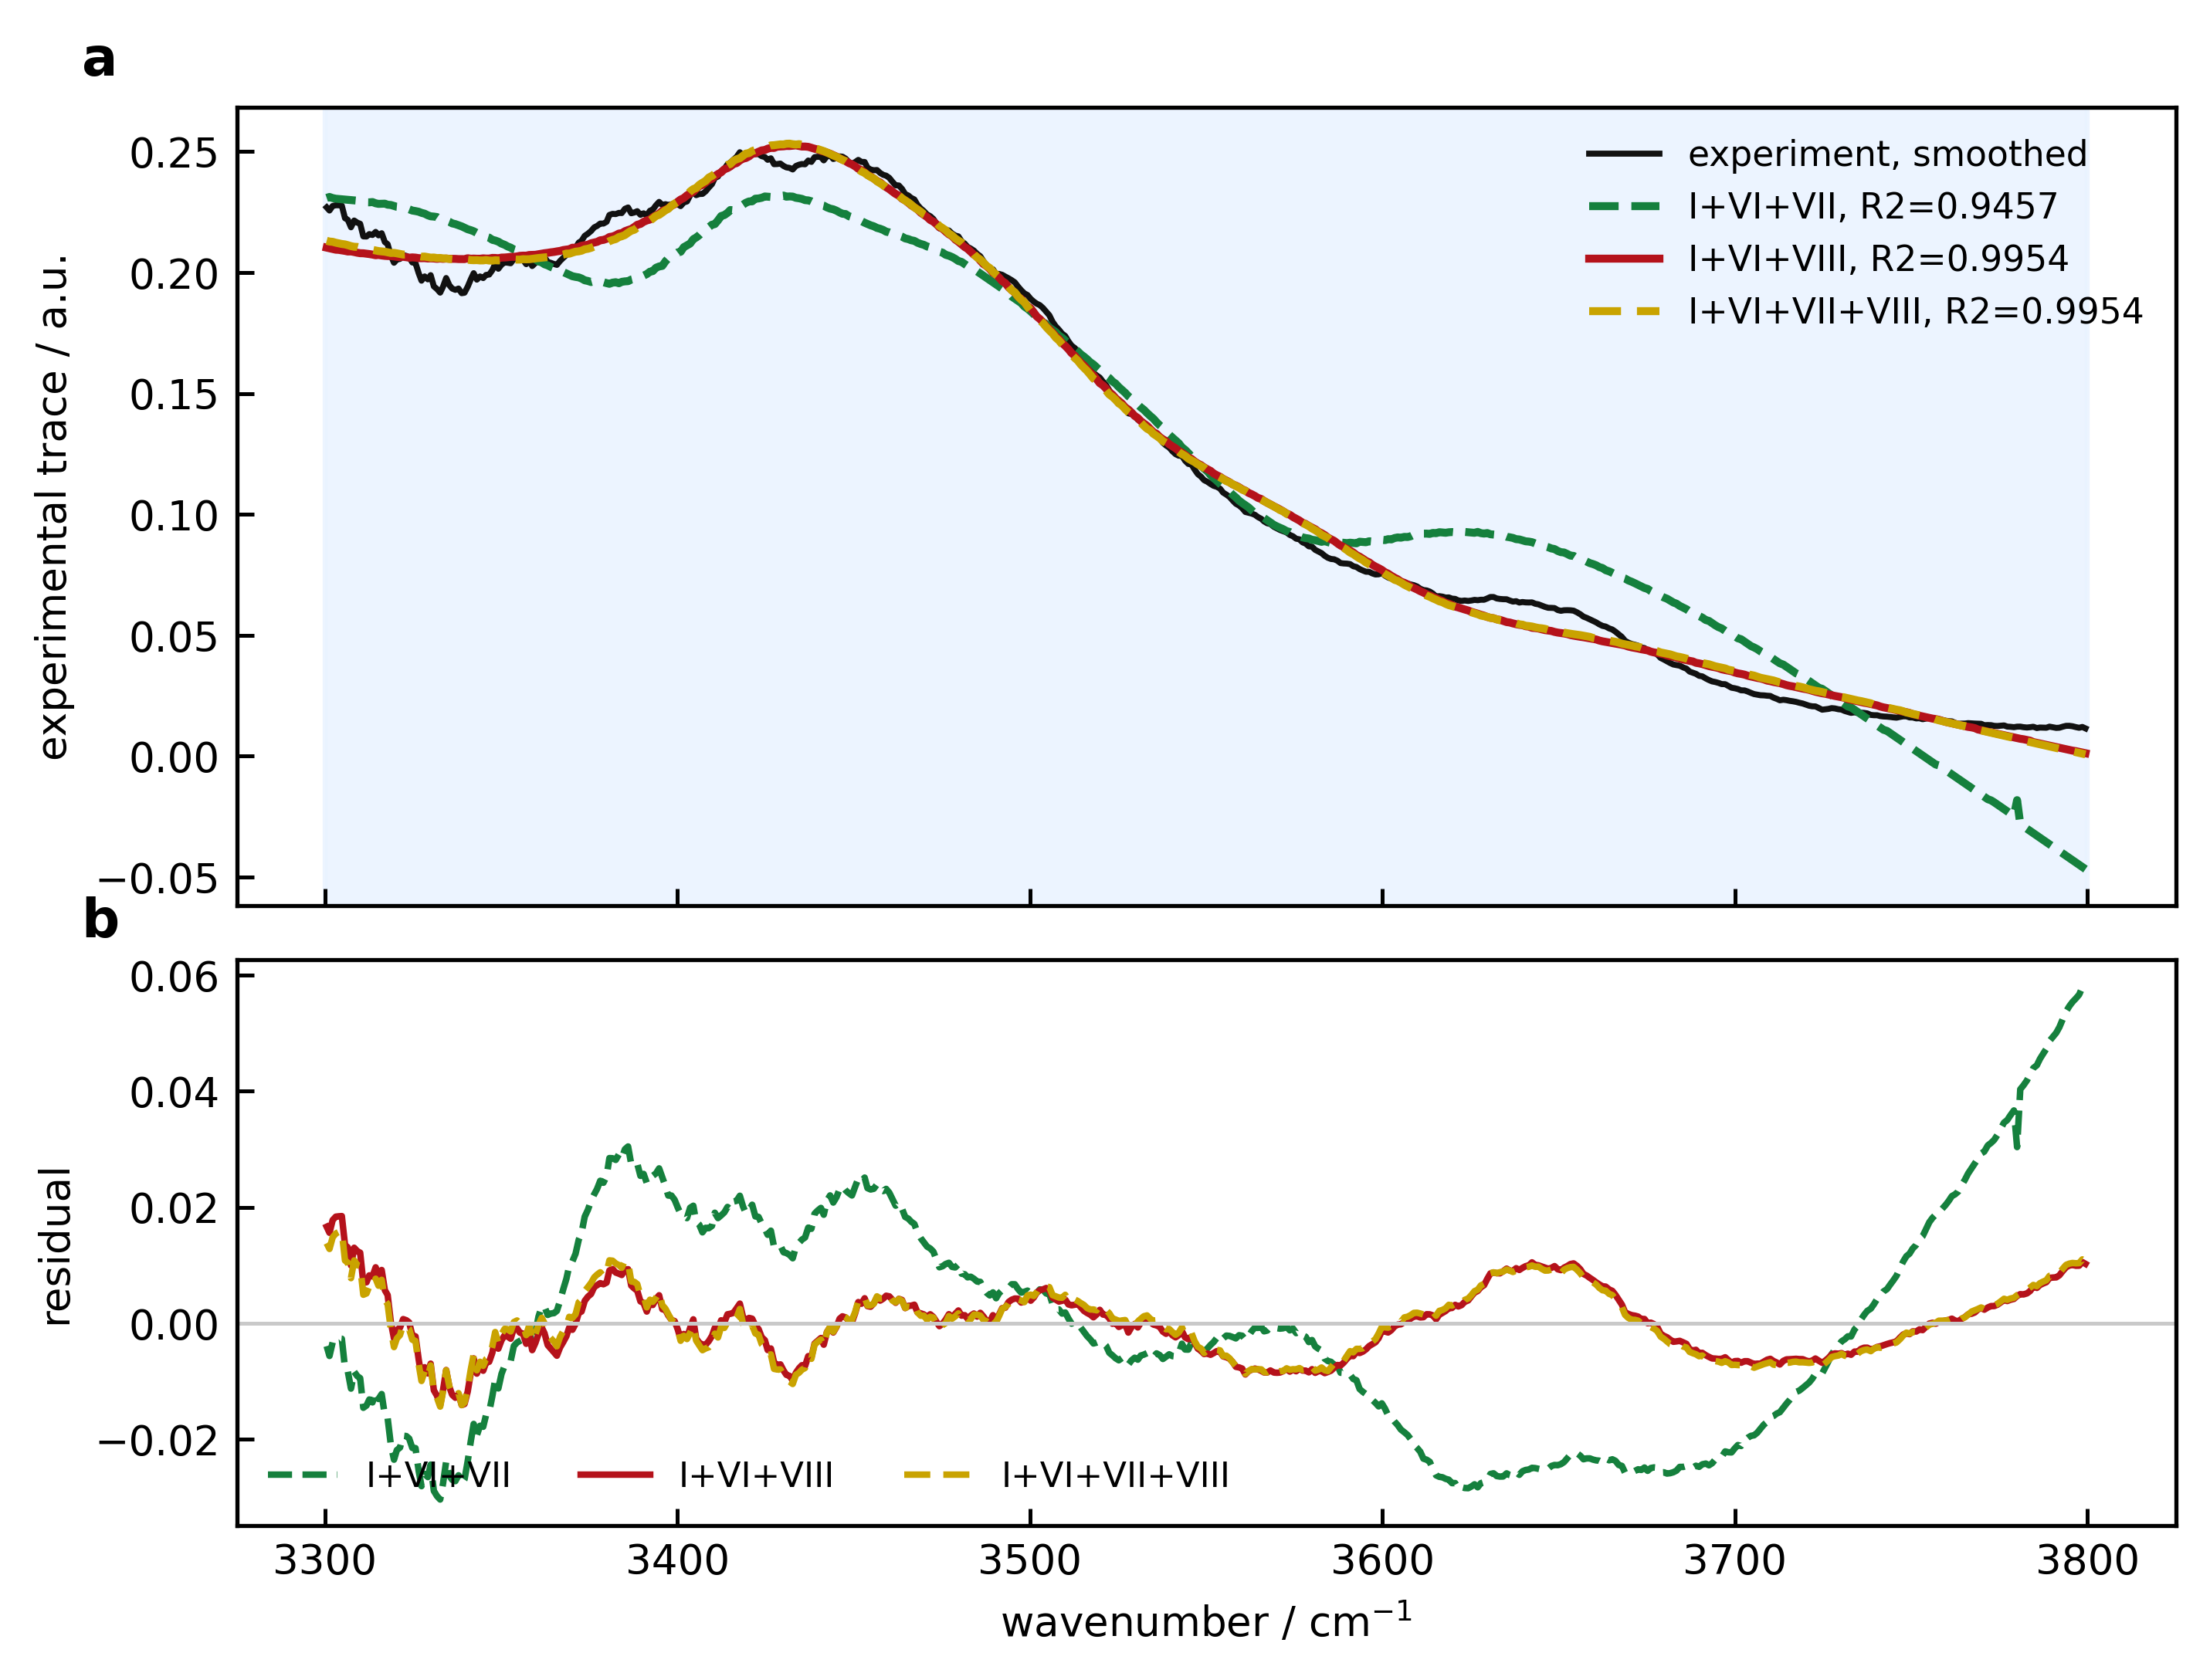
\includegraphics[width=0.92\textwidth]{figS_new_l3_vii_viii_control}
\caption{Direct L3-control fits in the primary physically interpretable \SIrange{3300}{3800}{cm^{-1}} OH-transfer window. A VII-only L3 substitution gives a substantially poorer fit, whereas adding VII to I+VI+VIII gives only a very small visual and numerical change.}
\end{figure}

\begin{table}[H]
\centering
\caption{Direct VII/VIII control in the primary physically interpretable \SIrange{3300}{3800}{cm^{-1}} OH-transfer window. The I+VI+VII fit collapses to a VI-only solution within the nonnegative least-squares constraint, whereas the I+VI+VIII and I+VI+VII+VIII fits are nearly indistinguishable.}
\begin{tabular}{lccccc}
\toprule
model & active motifs & $R^2$ & SSE & shift / \si{cm^{-1}} & BIC \\
\midrule
I+VI+VII & VI & 0.945677 & 0.223992 & -20 & -4323.4 \\
I+VI+VIII & I+VI+VIII & 0.995350 & 0.019173 & +4 & -5692.6 \\
I+VI+VII+VIII & I+VI+VII+VIII & 0.995433 & 0.018829 & +2 & -5696.3 \\
\bottomrule
\end{tabular}
\end{table}

This control does not prove that the microscopic L3 population is purely motif VIII. It shows that the dominant L3 response is assigned to motif VIII, while motif VII remains a symmetry-related/near-degenerate admixture that cannot be uniquely excluded from the one-dimensional SFG trace. Azimuthal mirror variants of a motif are likewise not expected to be cleanly resolved unless they change the OH orientation relative to the surface normal.

\section*{Exact Motif Candidate Fits}

\begin{figure}[H]
\centering
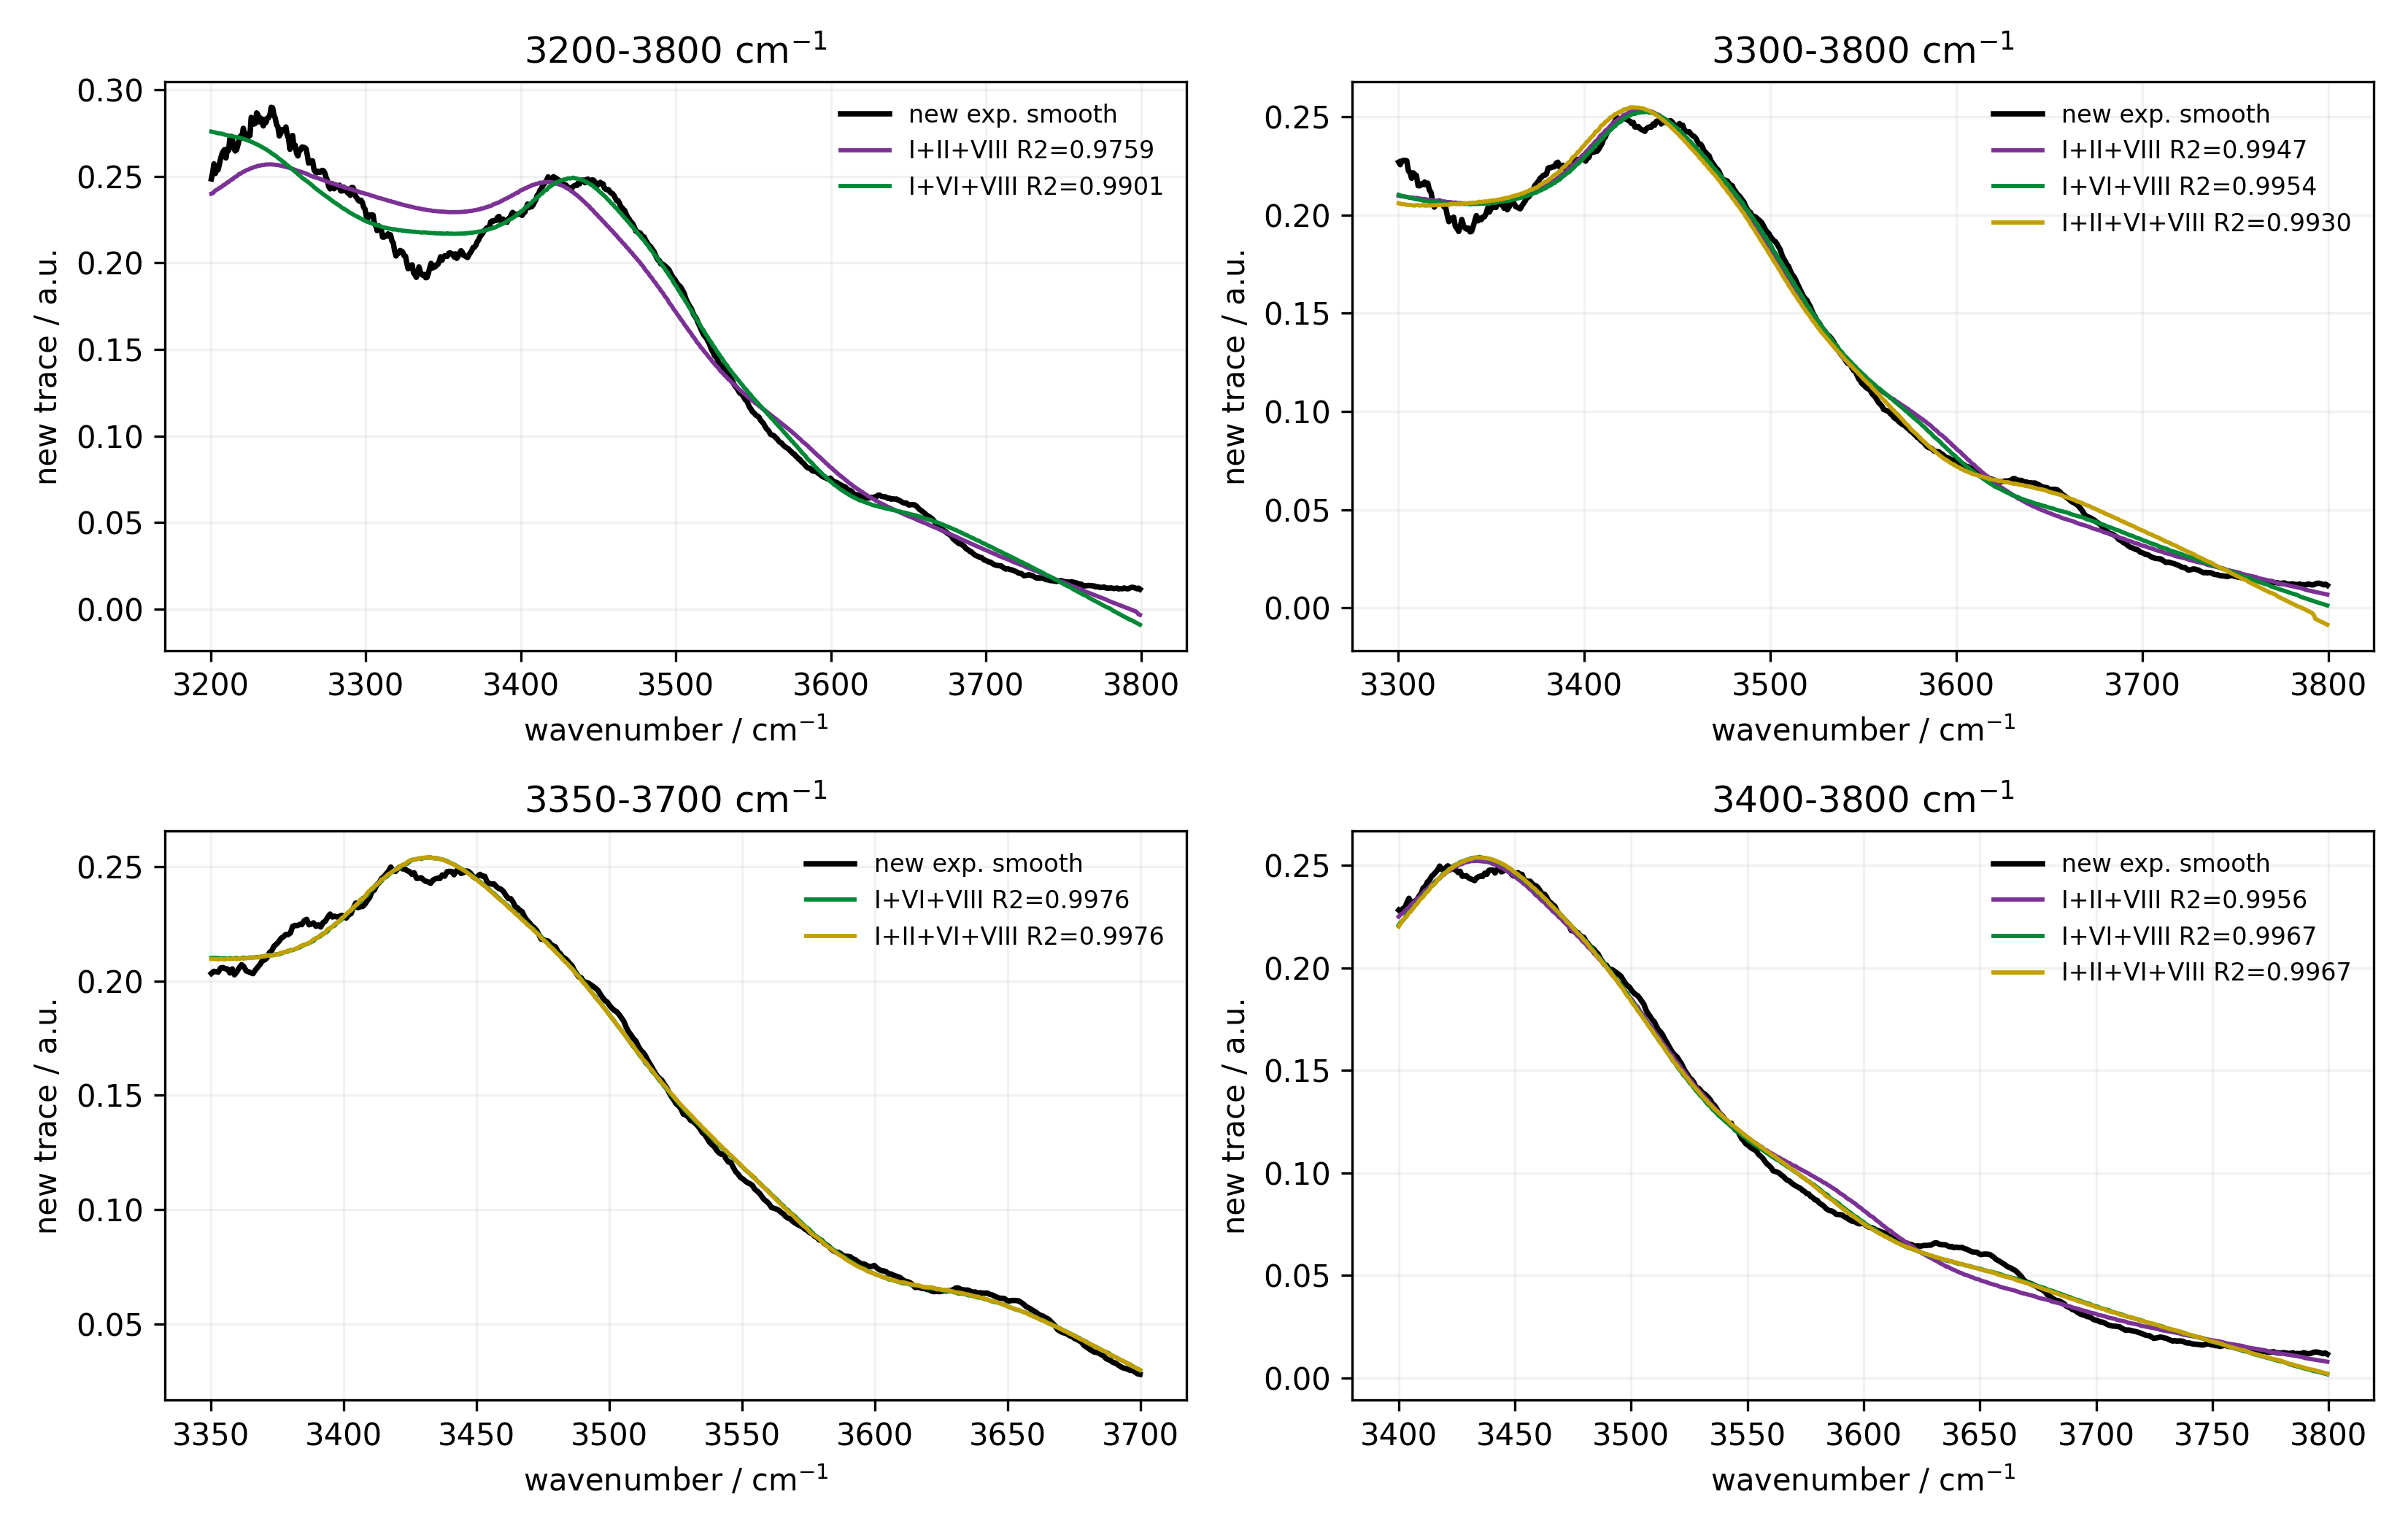
\includegraphics[width=0.95\textwidth]{figS_new_exact_motif_candidate_fits}
\caption{Selected exact motif fits in several spectral windows. The I+VI+VIII and I+VI+VII+VIII models are nearly indistinguishable in the primary physically interpretable \SIrange{3300}{3800}{cm^{-1}} OH-transfer window. In narrower high-frequency windows, several models can reach very high $R^2$, illustrating the underdetermined character of the inversion.}
\end{figure}

\begin{table}[H]
\centering
\caption{Exact motif-set selection for the two most relevant windows. The table reports fits with 17-point smoothing and a conservative shift range of \SI{\pm20}{cm^{-1}}.}
\begin{tabular}{lccccc}
\toprule
window / \si{cm^{-1}} & active motifs & $R^2$ & SSE & shift / \si{cm^{-1}} & BIC \\
\midrule
3300--3800 & I+VI+VII+VIII & 0.995433 & 0.018829 & +2 & -5696.3 \\
3300--3800 & I+VI+VIII & 0.995350 & 0.019173 & +4 & -5692.6 \\
3300--3800 & I+II+VIII & 0.994655 & 0.022038 & +7 & -5615.0 \\
3300--3800 & I+II+VI+VIII & 0.993007 & 0.028836 & -8 & -5458.9 \\
\midrule
3400--3800 & I+IV+VI+VIII & 0.996938 & 0.009599 & -5 & -4721.1 \\
3400--3800 & I+VI+VIII & 0.996677 & 0.010414 & +2 & -4691.1 \\
3400--3800 & I+II+VI+VIII & 0.996717 & 0.010291 & 0 & -4690.3 \\
3400--3800 & I+II+VIII & 0.995552 & 0.013942 & +9 & -4561.8 \\
\bottomrule
\end{tabular}
\end{table}

The \SIrange{3200}{3800}{cm^{-1}} window is useful diagnostically because it reveals low-edge sensitivity, while the \SIrange{3400}{3800}{cm^{-1}} high-frequency control can be fit very well by several related bridge-family models. This is why the main text emphasizes the \SIrange{3300}{3800}{cm^{-1}} primary physically interpretable OH-transfer window: it retains the high-frequency weak-OH region and the bonded OH response while avoiding the noisier low edge. Within that window, the I+VI+VIII model is the parsimonious three-motif interpretation, and motif VI is the preferred bridge-family connector.

\section*{Smoothing and Window Robustness}

\begin{figure}[H]
\centering
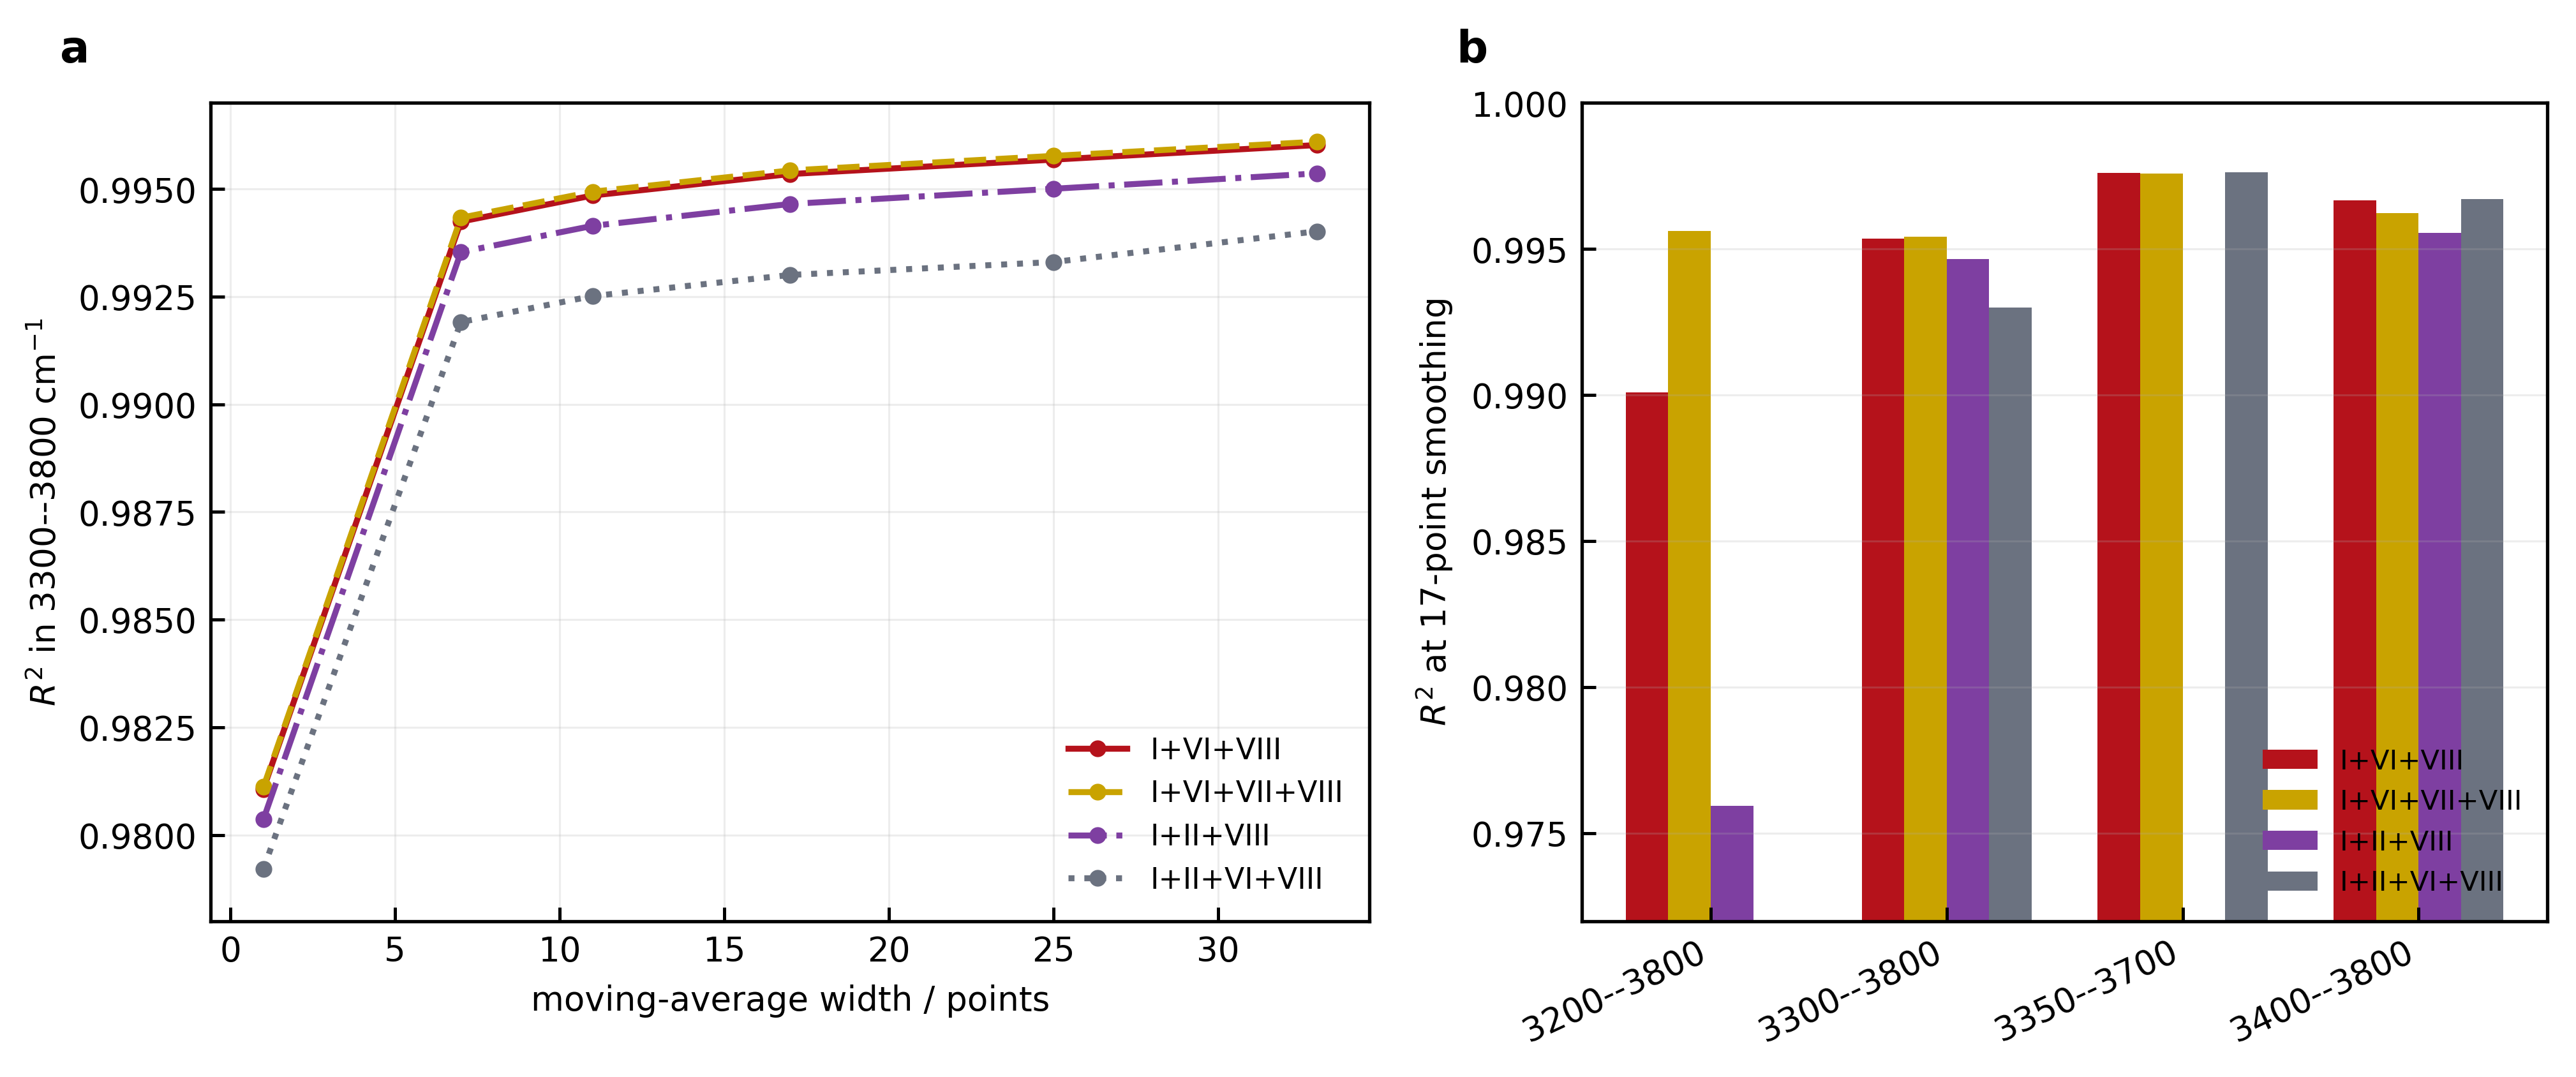
\includegraphics[width=0.96\textwidth]{figS_new_window_smoothing_robustness}
\caption{Robustness of selected model classes. (a) $R^2$ in the primary physically interpretable \SIrange{3300}{3800}{cm^{-1}} OH-transfer window as a function of moving-average width. (b) Window dependence at 17-point smoothing. The \SIrange{3200}{3800}{cm^{-1}} window is diagnostic for low-edge sensitivity, while the very high $R^2$ values in narrower or higher-frequency windows illustrate why window variation is a diagnostic for underdetermination rather than a route to a unique structure.}
\end{figure}

\begin{table}[H]
\centering
\caption{$R^2$ of the I+VI+VIII primary model as a function of smoothing window. The 17-point value is used in the main text.}
\begin{tabular}{lcccccc}
\toprule
fit window / \si{cm^{-1}} & 1 pt & 7 pt & 11 pt & 17 pt & 25 pt & 33 pt \\
\midrule
3300--3800 & 0.981067 & 0.994246 & 0.994852 & 0.995350 & 0.995685 & 0.996023 \\
3400--3800 & 0.990688 & 0.995927 & 0.996348 & 0.996677 & 0.996847 & 0.996977 \\
\bottomrule
\end{tabular}
\end{table}

\begin{table}[H]
\centering
\caption{$R^2$ robustness for selected competing models in the primary physically interpretable \SIrange{3300}{3800}{cm^{-1}} OH-transfer window.}
\begin{tabular}{lcccccc}
\toprule
model & 1 pt & 7 pt & 11 pt & 17 pt & 25 pt & 33 pt \\
\midrule
I+VI+VIII & 0.981067 & 0.994246 & 0.994852 & 0.995350 & 0.995685 & 0.996023 \\
I+VI+VII+VIII & 0.981112 & 0.994336 & 0.994939 & 0.995433 & 0.995772 & 0.996101 \\
I+II+VIII & 0.980364 & 0.993538 & 0.994147 & 0.994655 & 0.995008 & 0.995365 \\
I+II+VI+VIII & 0.979213 & 0.991913 & 0.992516 & 0.993007 & 0.993307 & 0.994020 \\
\bottomrule
\end{tabular}
\end{table}

The smoothing test shows that the qualitative conclusion is not a consequence of choosing exactly 17 points. The no-smoothing fits are lower because the raw trace contains high-frequency point noise, especially near the low edge. For all tested smoothing windows from 7 to 33 points, the I+VI+VIII and I+VI+VII+VIII models remain the strongest candidates in the primary OH-transfer window.

\section*{Machine-Readable Files}

The local project contains the numerical data used in this draft:

\begin{longtable}{p{0.36\textwidth}p{0.55\textwidth}}
\caption{Core numerical records for the analysis.}\\
\toprule
record & contents \\
\midrule
\endfirsthead
\toprule
record & contents \\
\midrule
\endhead
experimental trace & Frequency axis and measured response channel. \\
processed trace & Raw, interpolated, and smoothed forms of the trace. \\
primary fit curve & I+VI+VIII fit curve, baseline, residual, and component curves. \\
primary weights & Nonnegative weights and RMS fractions for the primary model. \\
model-selection diagnostics & Three-motif model, four-motif control, and candidate-model sensitivity. \\
window diagnostics & Data-internal window-quality diagnostics, including raw-minus-smoothed RMS values. \\
L3 controls & Fit and residual curves for direct VII/VIII controls in the primary OH-transfer window. \\
fingerprint basis & Digitized water--air Rosetta-stone fingerprints used as structural basis functions. \\
\bottomrule
\end{longtable}

\end{document}
